\def\year{2020}\relax
%File: formatting-instruction.tex
\documentclass[letterpaper]{article} % DO NOT CHANGE THIS
\usepackage{aaai20}  % DO NOT CHANGE THIS
\usepackage{times}  % DO NOT CHANGE THIS
\usepackage{helvet} % DO NOT CHANGE THIS
\usepackage{courier}  % DO NOT CHANGE THIS
\usepackage[hyphens]{url}  % DO NOT CHANGE THIS
\usepackage{graphicx} % DO NOT CHANGE THIS
\urlstyle{rm} % DO NOT CHANGE THIS
\def\UrlFont{\rm}  % DO NOT CHANGE THIS
\usepackage{graphicx}  % DO NOT CHANGE THIS
\frenchspacing  % DO NOT CHANGE THIS
\setlength{\pdfpagewidth}{8.5in}  % DO NOT CHANGE THIS
\setlength{\pdfpageheight}{11in}  % DO NOT CHANGE THIS
%\nocopyright
%PDF Info Is REQUIRED.
% For /Author, add all authors within the parentheses, separated by commas. No accents or commands.
% For /Title, add Title in Mixed Case. No accents or commands. Retain the parentheses.
 \pdfinfo{
/Title (AAAI Press Formatting Instructions for Authors Using LaTeX -- A Guide)
/Author (AAAI Press Staff, Pater Patel Schneider, Sunil Issar, J. Scott Penberthy, George Ferguson, Hans Guesgen)
} %Leave this	
% /Title ()
% Put your actual complete title (no codes, scripts, shortcuts, or LaTeX commands) within the parentheses in mixed case
% Leave the space between \Title and the beginning parenthesis alone
% /Author ()
% Put your actual complete list of authors (no codes, scripts, shortcuts, or LaTeX commands) within the parentheses in mixed case. 
% Each author should be only by a comma. If the name contains accents, remove them. If there are any LaTeX commands, 
% remove them. 

% DISALLOWED PACKAGES
% \usepackage{authblk} -- This package is specifically forbidden
% \usepackage{balance} -- This package is specifically forbidden
% \usepackage{caption} -- This package is specifically forbidden
% \usepackage{color (if used in text)
% \usepackage{CJK} -- This package is specifically forbidden
% \usepackage{float} -- This package is specifically forbidden
% \usepackage{flushend} -- This package is specifically forbidden
% \usepackage{fontenc} -- This package is specifically forbidden
% \usepackage{fullpage} -- This package is specifically forbidden
% \usepackage{geometry} -- This package is specifically forbidden
% \usepackage{grffile} -- This package is specifically forbidden
% \usepackage{hyperref} -- This package is specifically forbidden
% \usepackage{navigator} -- This package is specifically forbidden
% (or any other package that embeds links such as navigator or hyperref)
% \indentfirst} -- This package is specifically forbidden
% \layout} -- This package is specifically forbidden
% \multicol} -- This package is specifically forbidden
% \nameref} -- This package is specifically forbidden
% \natbib} -- This package is specifically forbidden -- use the following workaround:
% \usepackage{savetrees} -- This package is specifically forbidden
% \usepackage{setspace} -- This package is specifically forbidden
% \usepackage{stfloats} -- This package is specifically forbidden
% \usepackage{tabu} -- This package is specifically forbidden
% \usepackage{titlesec} -- This package is specifically forbidden
% \usepackage{tocbibind} -- This package is specifically forbidden
% \usepackage{ulem} -- This package is specifically forbidden
% \usepackage{wrapfig} -- This package is specifically forbidden
% DISALLOWED COMMANDS
% \nocopyright -- Your paper will not be published if you use this command
% \addtolength -- This command may not be used
% \balance -- This command may not be used
% \baselinestretch -- Your paper will not be published if you use this command
% \clearpage -- No page breaks of any kind may be used for the final version of your paper
% \columnsep -- This command may not be used
% \newpage -- No page breaks of any kind may be used for the final version of your paper
% \pagebreak -- No page breaks of any kind may be used for the final version of your paperr
% \pagestyle -- This command may not be used
% \tiny -- This is not an acceptable font size.
% \vspace{- -- No negative value may be used in proximity of a caption, figure, table, section, subsection, subsubsection, or reference
% \vskip{- -- No negative value may be used to alter spacing above or below a caption, figure, table, section, subsection, subsubsection, or reference

\setcounter{secnumdepth}{0} %May be changed to 1 or 2 if section numbers are desired.

% The file aaai20.sty is the style file for AAAI Press 
% proceedings, working notes, and technical reports.
%
\setlength\titlebox{2.5in} % If your paper contains an overfull \vbox too high warning at the beginning of the document, use this
% command to correct it. You may not alter the value below 2.5 in
\title{Hand Gesture Recognition Using Artificial Intelligence}
%Your title must be in mixed case, not sentence case. 
% That means all verbs (including short verbs like be, is, using,and go), 
% nouns, adverbs, adjectives should be capitalized, including both words in hyphenated terms, while
% articles, conjunctions, and prepositions are lower case unless they
% directly follow a colon or long dash
\author{\Large \textbf{Talal Siddiqui, Visheshank Mishra}\\ % All authors must be in the same font size and format. Use \Large and \textbf to achieve this result when breaking a line
%If you have multiple authors and multiple affiliations
% use superscripts in text and roman font to identify them. For example, Sunil Issar,\textsuperscript{\rm 2} J. Scott Penberthy\textsuperscript{\rm 3} George Ferguson,\textsuperscript{\rm 4} Hans Guesgen\textsuperscript{\rm 5}. Note that the comma should be placed BEFORE the superscript for optimum readability
Northeastern University\\
360 Huntington Ave, Boston, MA 021153\\
siddiqui.t@northeastern.edu, mishra.vis@northeastern.edu\\ % email address must be in roman text type, not monospace or sans serif
https://github.com/talals1/cs5100-final-project
}
 \begin{document}

\maketitle

\begin{abstract}
For our final project in CS5100: Foundations of Artificial Intelligence, we chose to research and implement a system that can recognize hand gestures via a webcam. To do this, we utilized several techniques in artificial intelligence and machine learning such as various classifiers, image segmentation, background subtraction, and more. Our code is located at \url{https://github.com/talals1/cs5100-final-project}.


\end{abstract}

\section{Introduction}
Humans have been interacting with technology in a myriad of ways over the past century. From levers, switches, buttons, and now touch displays, the way we interact has been a constant focus in how we design the machines we use in our everyday lives. Currently, it seems like the next evolution of human-computer interaction is focused on interacting with computers without physical touch, such as talking or gesturing instead of manually clicking a button or turning a switch. There are many products already used by many that emphasize wireless control, such as voice assistants like Siri by Apple or Alexa by Amazon. As well, many have begun to simple systems of gesture control, but many of these systems are just marketing gimmicks with no real value.

For our project, we attempted to figure out the ways we could utilize gestures in a way that was actually useful and easy to use. To do this, we trained several types of classifier models using Python, Scikit-Learn, and several other libraries. Then, we created a program that uses the video feed from your webcam to detect your hand gesture and then perform appropriate behavior based on it.

\section{Background}
In order to be able to make a computer understand that a certain type of image corresponds to a certain value, we had to utilize things called \textit{classifiers}. Classifiers can be defined as mathematical models or algorithms that can be used to classify a certain input to a certain output. There are several types of classifiers in the world of artificial intelligence (AI), and the ones we used are called \textit{K-Nearest Neighors}, \textit{LinearSVC}, and the \textit{Random Forest Classifier}. Classifiers belong to a subgroup of machine learning called \textit{supervised learning}, which is where you have data that has labels assigned to it and the model trains itself by learning how certain samples correspond to certain labels.

For gesture recognition, the that a system will be predicting off of is going to be a person in a real life situation. This means that though the user's hand will be in the image, there will also be a lot of other unimportant things in both the foreground and background of the image. This includes things like the body of the user, lights, their room, and basically anything else in the room. The hand is just a small part of the picture, and finding the hand can be a tricky adventure. In order to extract out certain parts or features of an image, researchers use a technique called \textit{image segmentation}. Image segmentation is where you apply filters and masks to an image in order to highlight specific objects present in the image. For example, you could use image segmentation in order to highlight all the humans in a picture.

In our case, we needed to use image segmentation in order to focus on the hand in the image. What we hand to do was to find a specific way to segment each frame from the user's webcam so that only the gesturing hand was the only thing being shown in the image. Along with that, we also played around with \textit{background subtraction}, which is where after you segment an image, you get rid of everything else in the image in order to end up with the piece of the image necessary to make predictions from. 

As you can see, training a model was the easy part for us. The main challenge lay in figuring out the right combinations of filters and masks that would transform the input from the camera into an acceptable piece of data that our classifier model could use to make a prediction.

\section{Related Work}
There has been a lot of work done in image and gesture recognition over these past decades. The early days of facial recognition could probably be thought of as the first generation of gesture recognition since a lot of systems were designed to guess what feeling is being portrayed on a particular face. 

One of the earliest widespread uses of object recognition in live video was pioneered by Paul Viola and Michael Jones who created the Viola-Jones object recognition.

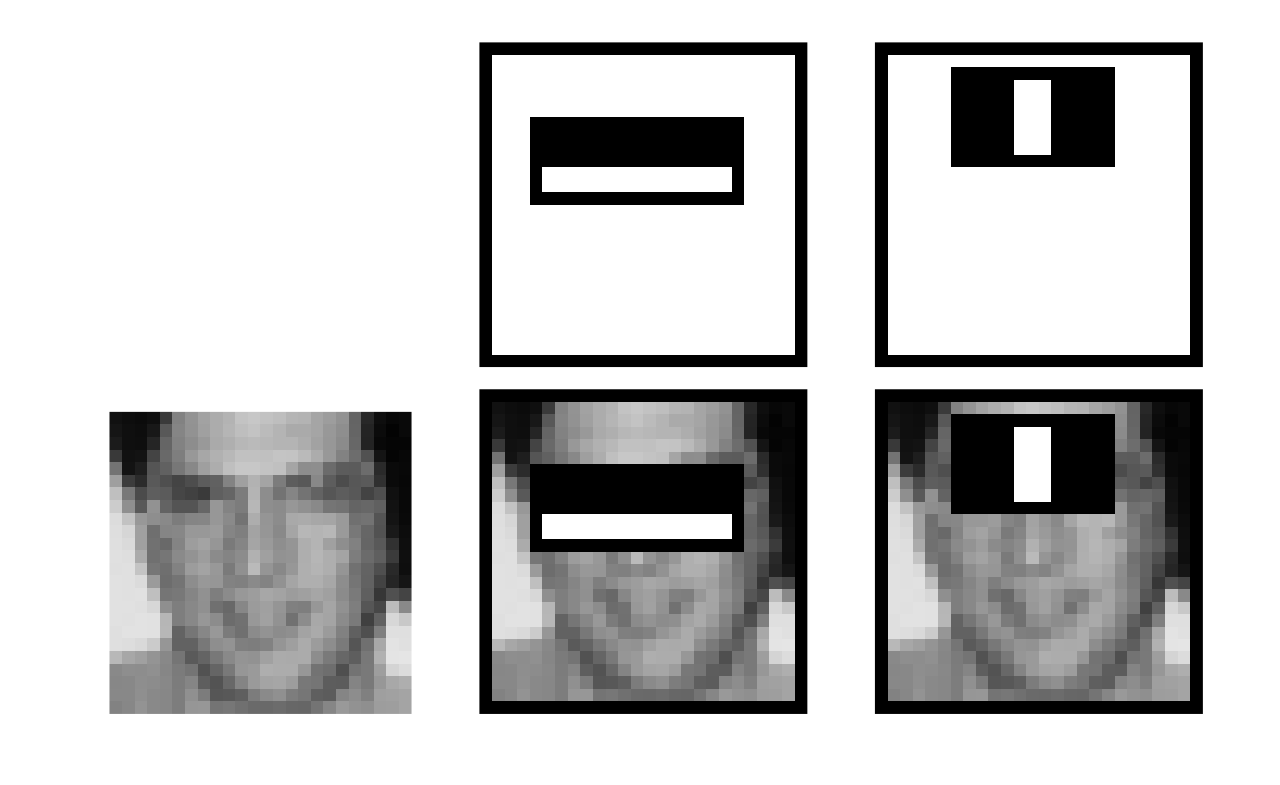
\includegraphics[scale=0.53]{violajones}

Above is a diagram of the Viola-Jones method, taken from their seminal paper "Robust Real-time Object Detection". The VJ method utilizes something called "features", which they describe as patterns they can use to detect whether or not a face is present in a particular area of a image. In the diagram above, we can see the features specific to a nose and to a upper cheek are being used to detect the mans face. This system was very widely used in cameras to detect faces for many years. Our approach is similar to this method as we also utilize a black and white representation of our image to identity an object (a hand gesture in our case). But unlike the VJ method, we do not scan over the entire image to detect our object since it seemed a bit complex for us.

The paper "A review of hand gesture and sign language recognition techniques" by Cheok, Omar, and Jawad goes over many techniques employed by various papers in detecting hand gestures. We particularly were interested in Cheok et al's description of using Hidden Markov Models (HMMs) in detecting hand gestures. But, we did not have much time to fully dive into HMMs and how they would be implemented to detect hand gestures for our project. Using HMMs may be an interesting way in detecting hand gestures, but the paper listed various ways that HMMs limitations cause its accuracy with hand gestures to hover at 90\% and below.

\section{Data Set Description}
We first began by finding a suitable dataset to use. There really isn't a whole lot of hand gesture datasets on the internet but we did first 2 on Kaggle that proved useful to us. The first one by someone named Arya R., which we term the "Simple Hand Set", was a collection of 50 by 50 pixel images that was quite simple since it did not have much data and because the images in the dataset were simple white and black pixels (no in-between values). 

The second dataset, which we term the "Complex Hand Set", is a collection of 150 by 150 pixel images that was taken via a Leap Motion camera by an group called "Gti". The complex hand set images were much more detailed and lifelike, which the simple hand dataset had images similar to pixel art since they were quite low resolution. In the end, we decided on using the complex data set since the models trained using the simple data set did not have a high accuracy when predicting off of the frames from our webcam, but more on that later.

The data set has the following gestures:

\begin{itemize}
	\item 1 = Palm
	\item 2 = L (right angle using index and thumb)
	\item 3 = Fist
	\item 4 = Fist at an angle
	\item 5 = Thumb
	\item 6 = Index finger
	\item 7 = OK sign
	\item 8 = Palm at an angle
	\item 9 = C (made using rounded index and thumb)
	\item 10 = Fingers pointing down
\end{itemize}


\section{Approach}
With out data sets in hand, we utilized Scikit-Learn's build in models for our classifiers. We used premade models instead of coding our own from scratch since the premade one are already very optimized, which means that nothing we could've made would've matched the performance of Sklearn's models.  

After we had trained a few models using the different classifiers previously mentioned, we put them to the test by making them predict live images from a webcam. To do this, we utilized the \textit{OpenCV} library in order to capture image from a webcam, apply filters, and then send it to the model. 

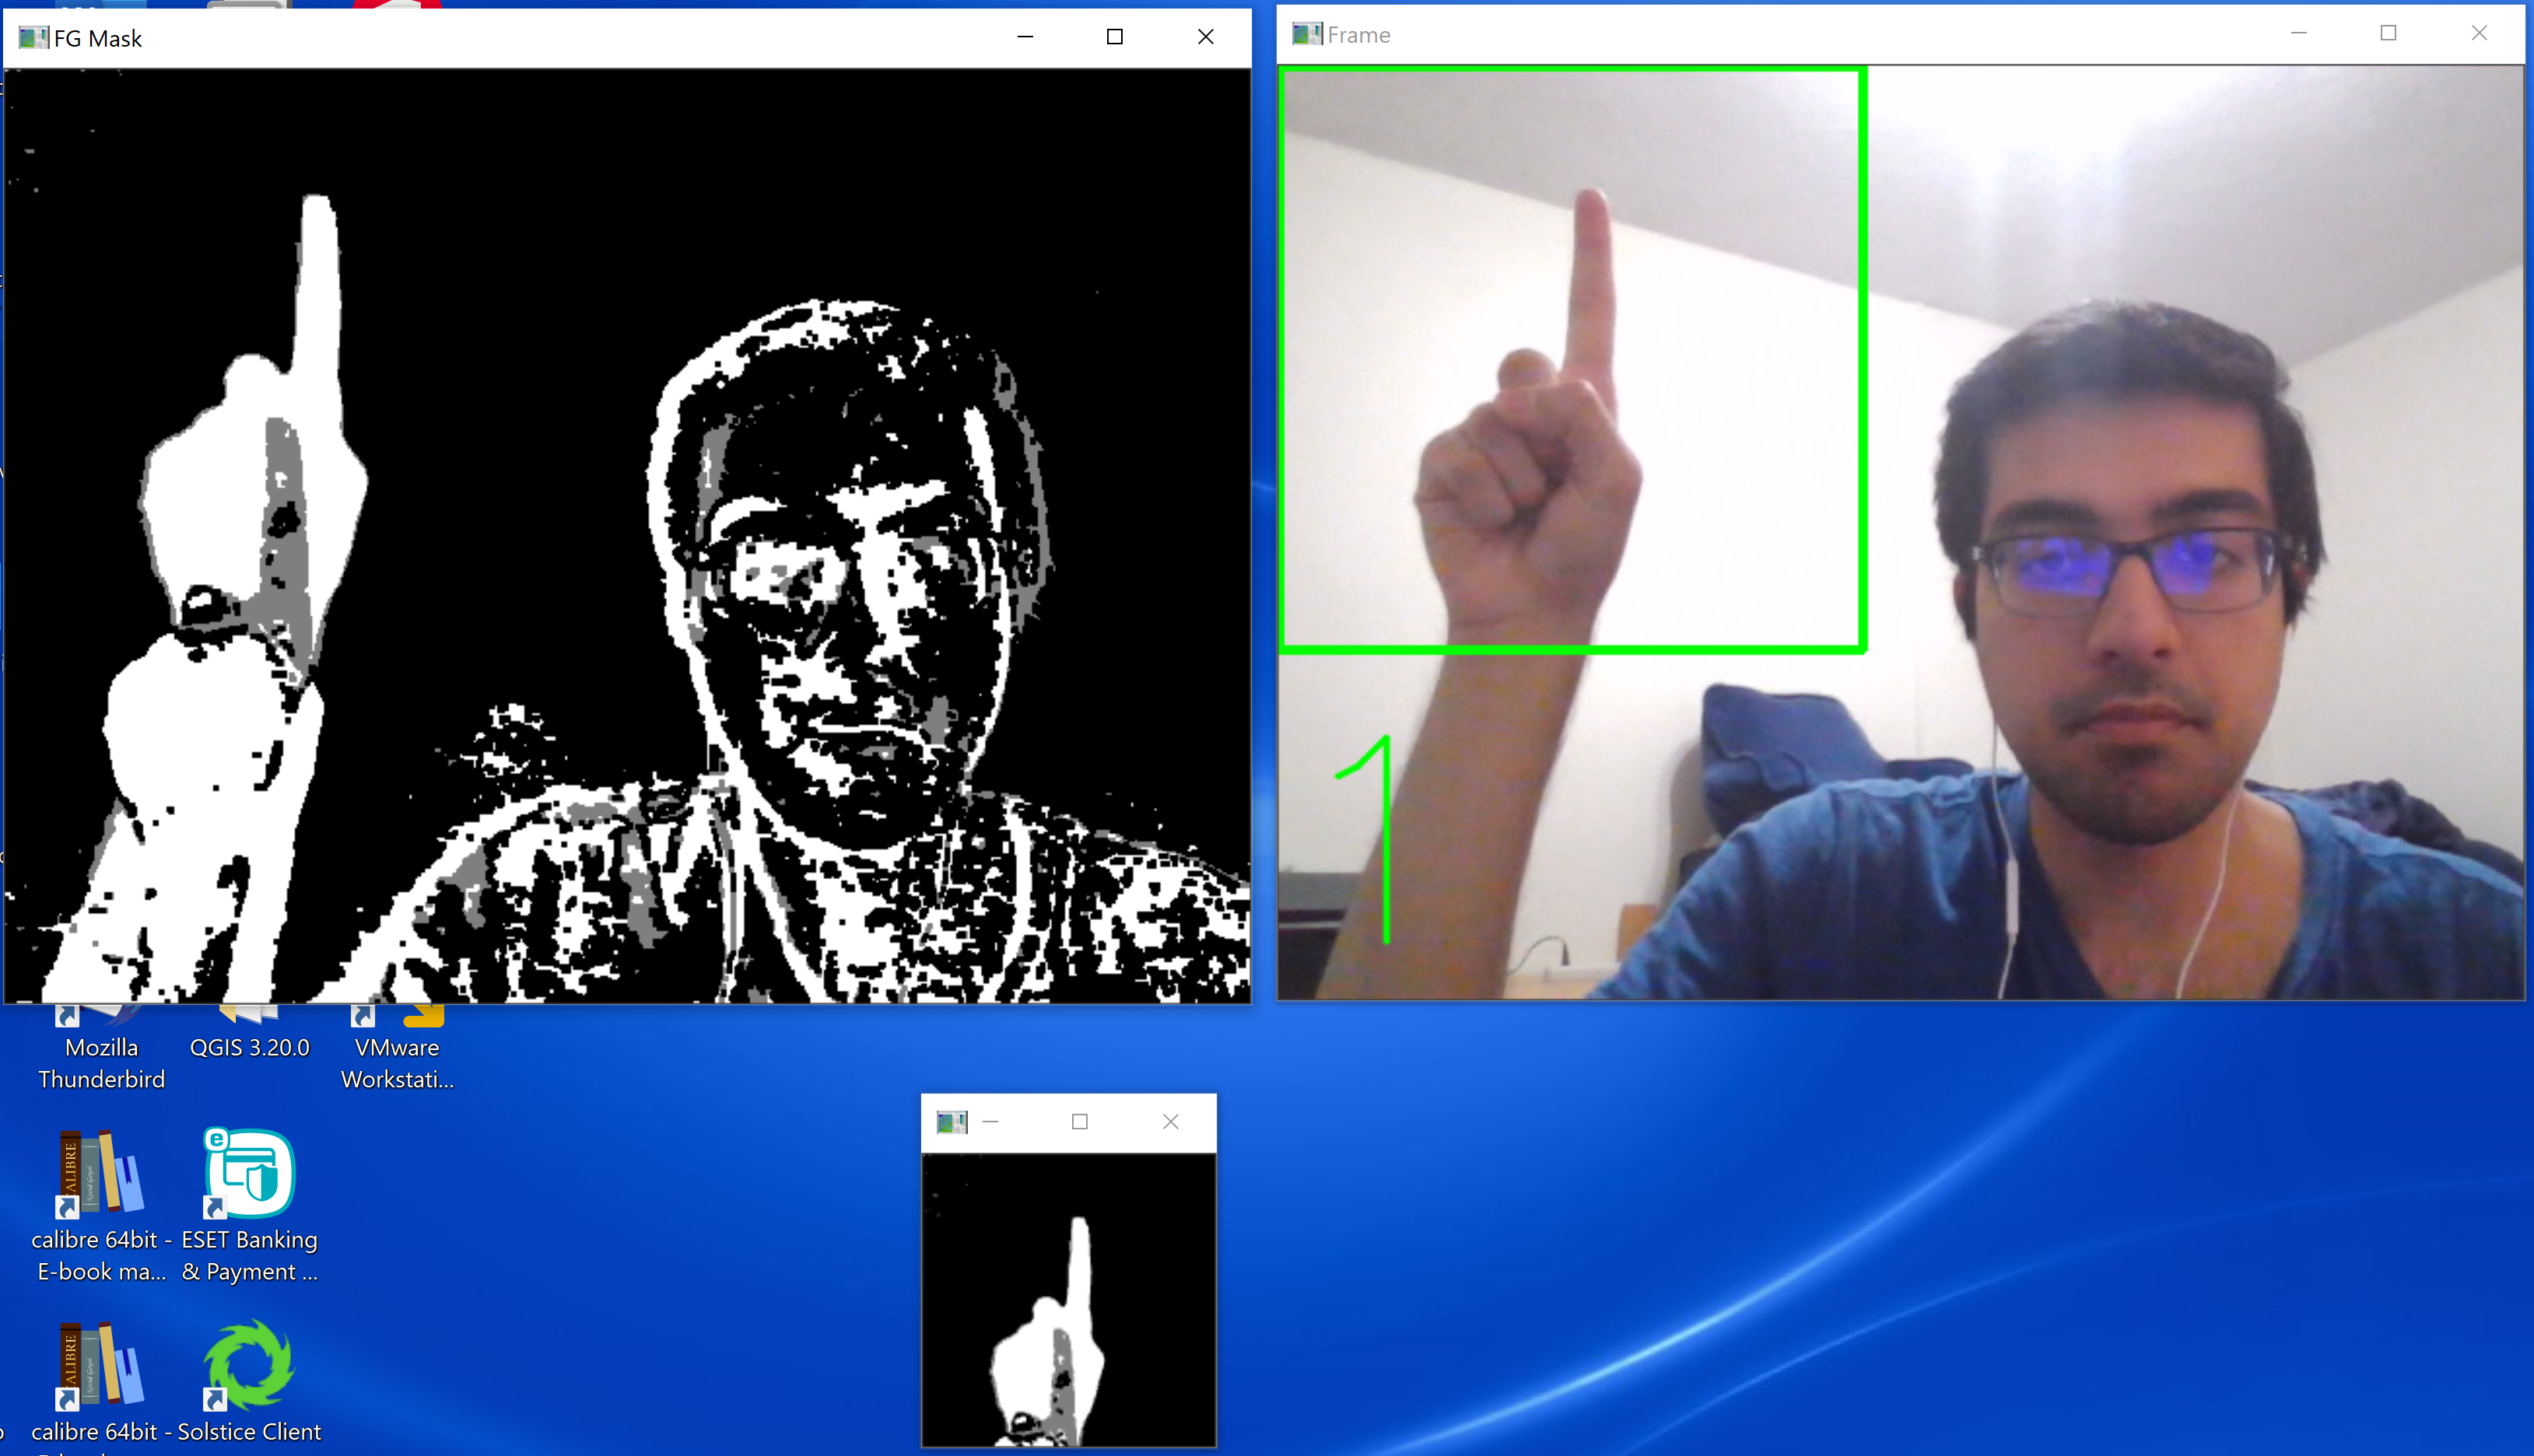
\includegraphics[scale=0.23]{handtest1}

Above is an image of the system in action. On the left is the full frame from the webcam after we processed it using a OpenCV's built-in image segmentation mask. The window on the right is what the user sees. The green box is there to tell the user where to put their hand gesture. We had considered making it so that the user could gesture anywhere in the image, but that proved to be too difficult since segmenting the image would run into too many artifacts and noise. Under the green box is a green number representing the models prediction. As you can see, the model is able to correctly predict that the user is gesture the number 1 to the camera.

Underneath the big 2 windows lies a small window in the center. The small window is what will be sent to the model for prediction. Its basically a cut out of the green square from the top right window. Before the frame is sent to the model, we flatten the matrix so it it becomes one contiguous array of data.


\section{Experiment and Results}

After training the model, the results seemed to be a bit confusing. When we had trained the model, we kept getting 100\% accuracy on the our classification matrix. As well, our confusion matrices seemed really good, as in we had little to none mis-classifications.

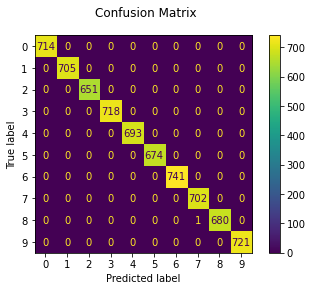
\includegraphics[scale=0.7]{complex-rfc-confusion}

Because of this, we decided to experiment with several different classifiers to see whether we weren't using the data and the models correctly or if we just had really good luck. We were afraid of a phenomenon called \textit{overfitting}, which is where a machine-learning system becomes so familiar with a given data set that it is 100\% accurate on the test and train sets. Overfitting is NOT a good thing since it is a signal that the model isn't really generalizing the features it detects in the data set and that it would not fair particularly well in the real world. Unfortunately, we did encounter something similar to that.
\\

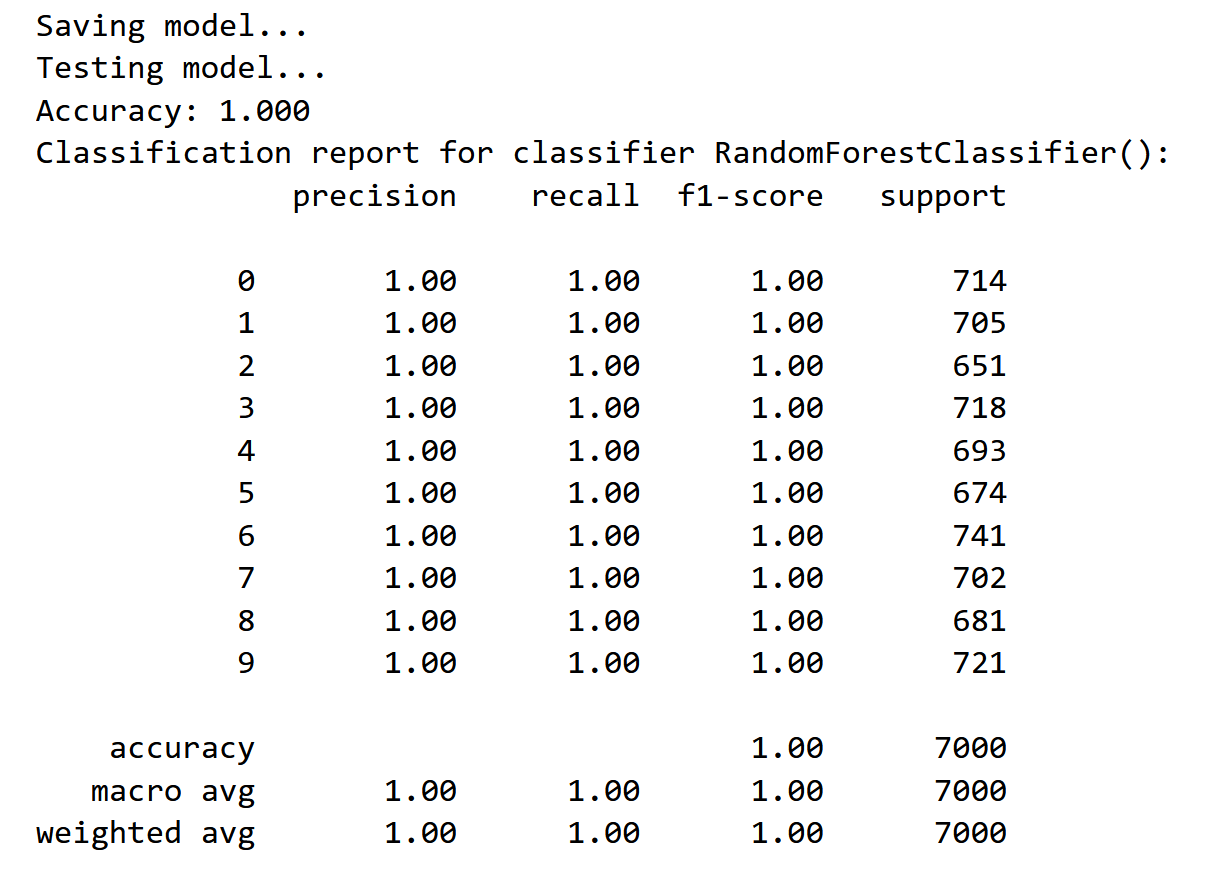
\includegraphics[scale=0.65]{complex-rfc-report}

As you can see above, the model seems to have 100\% accuracy after being tested on the testing data. However, when the model was utilized using live webcam feed, it performed quite poorly. It often would mis-classify gestures and would generally have a hard time getting its bearings straight. Since this was on real world data from our webcam, we were not able to collect much data about this. It would simplify mis-classify whenever we showed a gesture in the green box in the frame.
\\

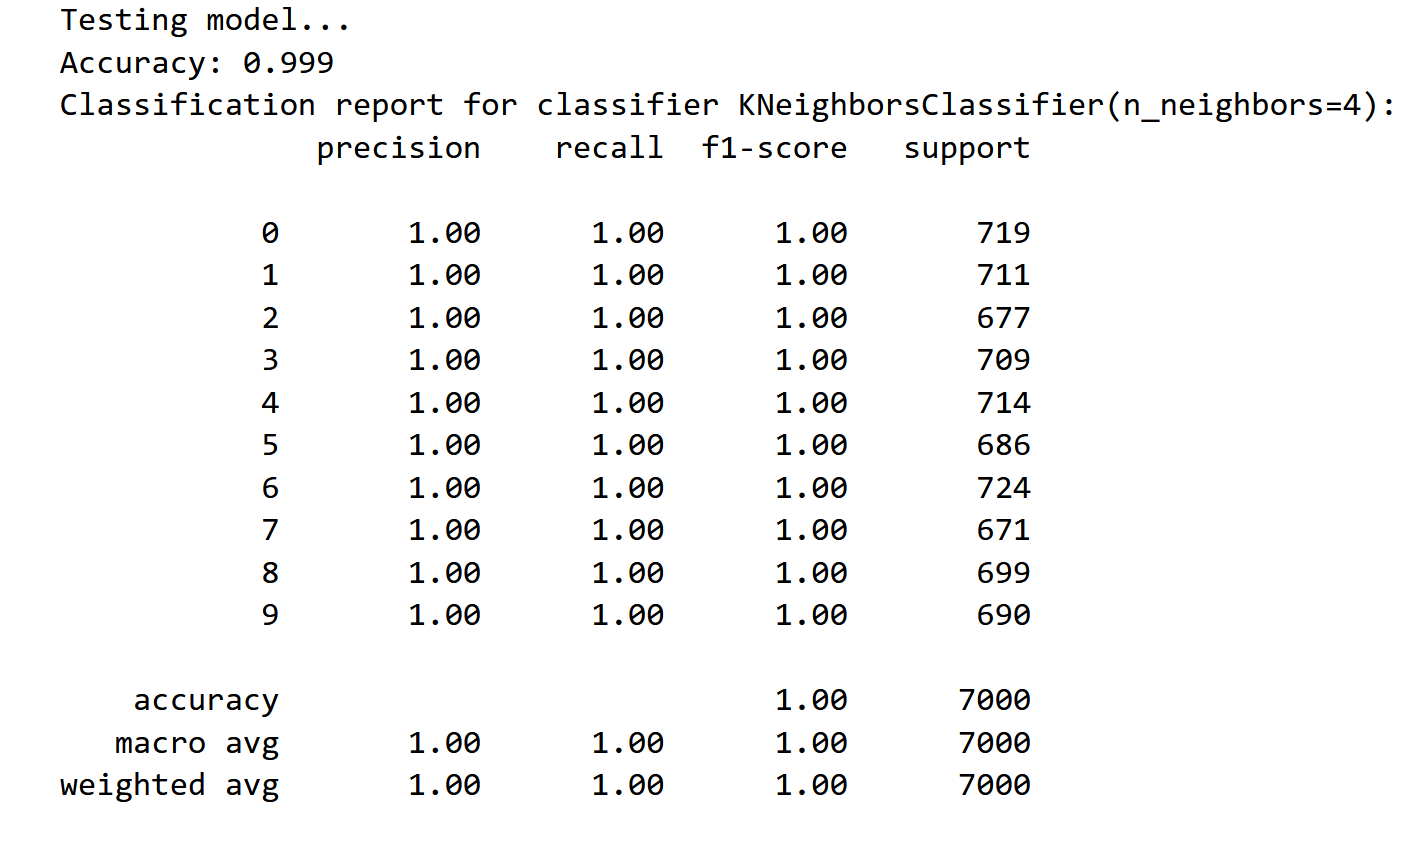
\includegraphics[scale=0.6]{complex-knn-report}

Above is the classification report for the K-Nearest Neighbors classifier. It too scored an almost perfect score, and had the same confusion matrix.

We believe that this sharp difference between the models performance in the testing data and via the webcam is mainly due to the way we had performed image segmentation and background subtraction. These 2 techniques are very hard to get right, and when you have a poor webcam, things do not get much easier. We often encountered a lot of noise in our images and had to spend a lot of time in making sure that only the designated hand region itself was extracted and sent to the model.

Overall the best gestures it could predict from the camera were 0, 1, and 2. Everything else wasn't quite impressive since they kept getting mis-classified by the model.

\section{Conclusion}
In conclusion, we believe we have created a foundation to a promising system. Though our models may have been overfitted, we believe that if we had better image segmentation, our model could have worked much better. 

Throughout this project, we learned so much about how much work really goes into image classification. Originally, we had assumed that image classification was just loading in images and throwing them at a neural network and calling it a day. But in reality, image classification has many parts that must work perfectly in conjunction with one another in order to get the best prediction from the model. As well, we learned that there is a long history of image classification, which we had assumed was a more recent phenomenon due to the perceived notion that this is the only time in history where computers were able to do anything insanely complex like identifying parts of an image.

We plan to look further into this project by enumerating all the possible ways that we could improve and fixing the parts that did not go exactly to plan. Hopefully, we plan to complete our vision of making a \textit{useful} hand gesture recognition system which could be used by anyone with a webcam.

\section{Future Scope}
Deep neural networks can be leveraged for our classification tasks, given enough training data these models can perform exceptionally well. Some of the models are AlexNet, VGG, ResNet, SqueezeNet, DenseNet Inception, GoogLeNet, ShuffleNet, MobileNet, MobileNet, ResNeXt, Wide ResNet, MNASNet, EfficientNet, RegNet, VisionTransformer, ConvNeXt. All of these have their own pros and cons, specifically in terms of memory, compute time, and performance.

Depending on the above-mentioned constraints, a suitable neural network can be trained for our classification task, upon which real-time classifications can be done in a certain fixed time interval, the output of this can be fed to another parallelly running process which can interpret the actions/operations to be performed via system calls of an OS. An example of this can be, A sequence of pre-defined hand gestures can activate volume control, followed by hand gestures depicting the a value of 0, 1, 2  to 10, which can correspond to the volume levels of 0\%, 10\%, 20\% to 100\%.


\section{References}

Arya, R. (2021, September 4). Hand gesture recognition dataset. Kaggle. Retrieved from https://www.kaggle.com/aryarishabh/hand-gesture-recognition-dataset 
\\

Gti. (2018, July 30). Hand gesture recognition database. Kaggle. Retrieved n.d., from https://www.kaggle.com/datasets/gti-upm/leapgestrecog
\\

cheok, ming jin, omar, zaid, Jaward, M. H. (2017, July 31). A review of hand gesture and sign language recognition techniques. Retrieved n.d., from https://www.researchgate.net/profile/Zaid-Omar-2/publication/318989820\_A\_review\_of\_hand\_gesture\_and\_
sign\_language\_recognition\_techniques/links/59d5be76aca272
5954c680de/A-review-of-hand-gesture-and-sign-language-recognition-techniques.pdf 
\\

Fang, Y., Wang, K., Cheng, J., Lu, H. (2007). A real-time hand gesture recognition method - IA. Retrieved from http://www.nlpr.ia.ac.cn/2007papers/gjhy/gh45.pdf 
\\

FastAI. (2022, January 20). Using the Learning Rate Finder (beginner). walkwithfastai. Retrieved n.d., from https://walkwithfastai.com/lr\_finder 
\\

Gogul Ilango. (2017, April 25). Hand gesture recognition using python and opencv - part 2. Gogul Ilango. Retrieved n.d., from https://gogul.dev/software/hand-gesture-recognition-p2 
\\

Gogul Ilango. (2017, April 6). Hand gesture recognition using python and opencv - part 1. Gogul Ilango. Retrieved n.d., from https://gogul.dev/software/hand-gesture-recognition-p1 
\\

Huang1, H., Chong2, Y., Nie2, C., Pan2, S. (2019, June 1). IOPscience. Journal of Physics: Conference Series. Retrieved n.d., from https://iopscience.iop.org/article/10.1088/1742-6596/1213/2/022001 
\\

Kostas, M. (2019, February 19). Understanding FASTAI's fit\_one\_cycle method. IconOf.com. Retrieved n.d., from https://iconof.com/1cycle-learning-rate-policy/ 
\\

Nausheen. (2021, February 11). Compute Performance Metrics-F1 score, precision, accuracy for CNN in fastai. Medium. Retrieved from https://towardsdev.com/compute-performance-metrics-f1-score-precision-accuracy-for-cnn-in-fastai-959d86b6f8ad 
\\

Synced. (2017, April 29). How to train a very large and deep model on one GPU? Medium. Retrieved n.d., from https://medium.com/syncedreview/how-to-train-a-very-large-and-deep-model-on-one-gpu-7b7edfe2d072 
\\

Viola, P., Jones, M. (2001). Rapid object detection using a boosted cascade of Simple features. CiteSeerX. Retrieved from http://citeseerx.ist.psu.edu/viewdoc/summary?doi=10.1.1.10.6807 
\\

Vision.transform. fastai. (2021, January 5). Retrieved n.d., from https://fastai1.fast.ai/vision.transform.html
%
%\smallskip \noindent \textit{Book with Multiple Authors}\\
%Engelmore, R., and Morgan, A. eds. 1986. \textit{Blackboard Systems.} Reading, Mass.: Addison-Wesley.
%
%\smallskip \noindent \textit{Journal Article}\\
%Robinson, A. L. 1980a. New Ways to Make Microcircuits Smaller. \textit{Science} 208: 1019--1026.
%
%\smallskip \noindent \textit{Magazine Article}\\
%Hasling, D. W.; Clancey, W. J.; and Rennels, G. R. 1983. Strategic Explanations in Consultation. \textit{The International Journal of Man-Machine Studies} 20(1): 3--19.
%
%\smallskip \noindent \textit{Proceedings Paper Published by a Society}\\
%Clancey, W. J. 1983. Communication, Simulation, and Intelligent Agents: Implications of Personal Intelligent Machines for Medical Education. In \textit{Proceedings of the Eighth International Joint Conference on Artificial Intelligence,} 556--560. Menlo Park, Calif.: International Joint Conferences on Artificial Intelligence, Inc.
%
%\smallskip \noindent \textit{Proceedings Paper Published by a Press or Publisher}\\
%Clancey, W. J. 1984. Classification Problem Solving. In \textit{Proceedings of the Fourth National Conference on Artificial Intelligence,} 49--54. Menlo Park, Calif.: AAAI Press. 
%
%\smallskip \noindent \textit{University Technical Report}\\
%Rice, J. 1986. Poligon: A System for Parallel Problem Solving, Technical Report, KSL-86-19, Dept. of Computer Science, Stanford Univ. 
%
%\smallskip \noindent \textit{Dissertation or Thesis}\\
%Clancey, W. J. 1979. Transfer of Rule-Based Expertise through a Tutorial Dialogue. Ph.D. diss., Dept. of Computer Science, Stanford Univ., Stanford, Calif.
%
%\smallskip \noindent \textit{Forthcoming Publication}\\
%Clancey, W. J. 2021. The Engineering of Qualitative Models. Forthcoming.



%\bibliography{refs.bib}{}
%\bibliographystyle{aaai} 

\end{document}
